\documentclass[12pt]{article}

% a template that a friend gave, it's worked well enough for me
% i have added some packages and stuff that have proved useful

\usepackage{fancyhdr}
\usepackage{tipa}
\usepackage{fontspec}
\usepackage{amsfonts}
\usepackage{enumitem}
\usepackage[margin=1in]{geometry}
\usepackage{graphicx}
\usepackage{float}
\usepackage{amsmath}
\usepackage{braket}
\usepackage{amssymb}
\usepackage{booktabs}
\usepackage{hyperref}
\usepackage{mathtools}
\usepackage{xcolor}
\usepackage{float}
\usepackage{algpseudocodex}
\usepackage{titlesec}
\usepackage{bbm}

\pagestyle{fancy}
\fancyhf{} % sets both header and footer to nothing
\lhead{Kevin Sheng}
\setmainfont{Comic Neue}
\renewcommand{\headrulewidth}{1pt}
\setlength{\headheight}{0.75in}
\setlength{\oddsidemargin}{0in}
\setlength{\evensidemargin}{0in}
\setlength{\voffset}{-.5in}
\setlength{\headsep}{10pt}
\setlength{\textwidth}{6.5in}
\setlength{\headwidth}{6.5in}
\setlength{\textheight}{8in}
\renewcommand{\headrulewidth}{0.5pt}
\renewcommand{\footrulewidth}{0.3pt}
\setlength{\textwidth}{6.5in}
\usepackage{setspace}
\usepackage{multicol}
\usepackage{float}
\setlength{\columnsep}{1cm}
\setlength\parindent{24pt}
\usepackage [english]{babel}
\usepackage [autostyle, english = american]{csquotes}
\MakeOuterQuote{"}

\setlength{\parskip}{6pt}
\setlength{\parindent}{0pt}

\titlespacing\section{0pt}{12pt plus 4pt minus 2pt}{0pt plus 2pt minus 2pt}
\titlespacing\subsection{0pt}{12pt plus 4pt minus 2pt}{0pt plus 2pt minus 2pt}
\titlespacing\subsubsection{0pt}{12pt plus 4pt minus 2pt}{0pt plus 2pt minus 2pt}

\hypersetup{colorlinks=true, urlcolor=blue}

\newcommand{\correction}[1]{\textcolor{red}{#1}}


\rhead{ECE 102}

\newcommand{\rect}{\operatorname{rect}}
\newcommand{\sinc}{\operatorname{sinc}}
\newcommand{\ft}[1]{\mathcal{F}\left[#1\right]}
\newcommand{\ift}[1]{\mathcal{F}^{-1}\left[#1\right]}

\begin{document}
\begin{enumerate}
      \item \begin{enumerate}
                  \item \begin{enumerate}
                              \item $Y(j\omega)=H(j\omega)X(j\omega)$, so it remains to find $\frac{Y(j\omega)}{X(j\omega)}$.
                                    We do this by taking the FTs of both sides of the differential equation.
                                    \begin{gather*}
                                          \mathcal{F}[y''(t)]+5\mathcal{F}[y'(t)]+6\mathcal{F}[y(t)]=3\mathcal{F}[x(t)] \\
                                          -\omega^2\mathcal{F}[y(t)]+5j\omega\mathcal{F}[y(t)]+6\mathcal{F}[y(t)]=3\mathcal{F}[x(t)] \\
                                          (-\omega^2+5j\omega+6)Y(j\omega)=3X(j\omega) \\
                                          H(j\omega)=\frac{Y(j\omega)}{X(j\omega)}=\boxed{\frac{3}{-\omega^2+5j\omega+6}}
                                    \end{gather*}
                              \item We first derive $\mathcal{F}[y_1(t)]$ and $Y(j\omega)$ to get $H_2$:
                                    \begin{align*}
                                          \mathcal{F}[y_1(t)] & =\frac{2}{1+j\omega}\text{ (derived in class)}                            \\
                                          \mathcal{F}[y(t)]
                                                              & =4\mathcal{F}\left[e^{-t}u(t)\right]-2\mathcal{F}\left[e^{-2t}u(t)\right] \\
                                                              & = \frac{4}{1+j\omega}-\frac{2}{2+j\omega}
                                    \end{align*}
                                    $Y(j\omega)=H_1(j\omega)H_2(j\omega)X(j\omega)$, so
                                    \begin{align*}
                                          H_2(j\omega)          & = \frac{Y(j\omega)}{H_1(j\omega)X(j\omega)}                           \\
                                                                & = \frac{\mathcal{F}[y(t)]}{\mathcal{F}[y_1(t)]}                       \\
                                                                & = \frac{\frac{4}{1+j\omega}-\frac{2}{2+j\omega}}{\frac{2}{1+j\omega}} \\
                                          \Aboxed{H_2(j\omega ) & = \frac{3+j\omega}{2+j\omega}}                                        \\
                                          H_1(j\omega)          & = \frac{H(j\omega)}{H_2(j\omega)}                                     \\
                                                                & = \frac{3}{-\omega^2+5j\omega+6} \div \frac{3+j\omega}{2+j\omega}     \\
                                          \Aboxed{H_1(j\omega)  & = \frac{3}{(3+j\omega)^2}}
                                    \end{align*}
                              \item \[\begin{aligned}
                                                \ift{H_1(j\omega)} & = \boxed{3te^{-3t}u(t)}                                 \\
                                                \ift{H_2(j\omega)} & = \ift{1}+\ift{\frac{1}{2+j\omega}}                     \\
                                                                   & = \boxed{\delta(t)+e^{-2t}u(t)}                         \\
                                                \ift{H(j\omega)}   & = \ift{\frac{3}{j\omega+2}-\frac{3}{j\omega+3}}         \\
                                                                   & = 3\ift{\frac{1}{j\omega+2}}-3\ift{\frac{1}{j\omega+3}} \\
                                                                   & = 3e^{-2t}u(t)-3e^{-3t}u(t)                             \\
                                                                   & = \boxed{3u(t)\left(e^{-2t}-e^{-3t}\right)}
                                          \end{aligned}\]
                        \end{enumerate}
                  \item Putting $x(t)$ through an LTI system is the same as convolving it with some $h(t)$
                        which is the same as multiplying $X(j\omega)$ with some $H(j\omega)$.

                        Because $X(j\omega)=0\ \forall |\omega|>\omega_0$,
                        $Y(j\omega)=X(j\omega)H(j\omega)=0\ \forall |\omega|>\omega_0$ as well.
                        Thus, $y(t)$ will only have a subset of the frequency components of $x(t)$.

                        This does not hold if we process $x(t)$ through a non-LTI system.
                        A counterexample could be a $\mathcal{S}[x(t)]=\delta(t)$,
                        since the FT of that is $1$ for all $t$.
                  \item We find the FTs of these systems' impulse responses.

                        For the first system,
                        $\ft{\rect\left(\frac{t}{\pi}\right)}=\pi\sinc\left(\frac{\omega}{2}\right)$,
                        so by duality
                        \[\ft{\sinc\left(\frac{t}{2}\right)}=2\rect\left(\frac{\omega}{\pi}\right)\]

                        Now we apply the modulation property to calculate $H_1(j\omega)$:
                        \begin{align*}
                              H_1(j\omega)
                               & = \ft{\sinc\left(\frac{t}{2}\right)\cos(\pi t)}                                                           \\
                               & = \frac{1}{2}\left(2\rect\left(\frac{\omega}{\pi}-1\right)+2\rect\left(\frac{\omega}{\pi}+1\right)\right) \\
                               & = \rect\left(\frac{\omega}{\pi}-1\right)+\rect\left(\frac{\omega}{\pi}+1\right)
                        \end{align*}

                        For the second system, by the same principles we have
                        $\ft{2\sinc(2t)}=\rect\left(\frac{\omega}{4\pi}\right)$.

                        Notice that these FTs are strictly real and nonnegative,
                        so their phase is $0$ and their magnitude is themselves.

                        Using a trig identity on $x(t)$ we have
                        \[x(t)=\cos(3\pi t)\cos(4\pi t)=\frac{\cos(7\pi t)+\cos(\pi t)}{2}\]

                        Splitting this into two cosines and using the hint gives us
                        \begin{align*}
                              (h_1 * x)(t)
                               & = |H_1(j(7\pi))| \cdot \frac{\cos(7\pi t)}{2}+|H_1(j\pi)| \cdot \frac{\cos(\pi t)}{2} \\
                               & = \boxed{\frac{\cos(\pi t)}{2}}
                        \end{align*}
                        for $h_1$
                        \begin{align*}
                              (h_2 * x)(t)
                               & = |H_2(j(7\pi))| \cdot \frac{\cos(7\pi t)}{2}+|H_2(j\pi)| \cdot \frac{\cos(\pi t)}{2} \\
                               & = \boxed{\frac{\cos(\pi t)}{2}}
                        \end{align*}
                        for $h_2$.

                        Unfortunately, not all input-output pairs can allow us
                        to deduce the system.
                        For example, all LTI systems give $y(t)=0$ in response to $x(t)=0$.
            \end{enumerate}
      \item \begin{enumerate}
                  \item We want the frequencies in the low-pass filter to destructively interfere, so $\alpha=-1$.
                        This does have a side effect of adding $\pi$ to the phase for all frequencies.
                  \item Ideal filters are non-realizable because they require convolution
                        with an infinite function that never really stops changing and isn't causal.
                  \item We just have to solve this system:
                        \begin{align*}
                              \frac{k}{\beta}=1 &  & \left|\frac{k}{\beta+2\pi j}\right|=\frac{1}{\sqrt{2}}
                        \end{align*}
                        The first equation allows us to say $\beta=k$, leaving only the second one.
                        I assumed $k$ was real and it led me to a valid solution, so:
                        \begin{gather*}
                              \left|\frac{k}{k+2\pi j}\right|=\frac{1}{\sqrt{2}} \\
                              \left|\frac{k(k-2\pi j)}{k^2+4\pi^2}\right|=\frac{1}{\sqrt{2}} \\
                              \frac{k^4}{\left(k^2+4\pi^2\right)^2}+\frac{4\pi^2k^2}{\left(k^2+4\pi^2\right)^2}=\frac{1}{2} \\
                              2k^4+8k^2\pi^2=\left(k^2+4\pi^2\right)^2 \\
                              k^4=16\pi^4 \\
                              \boxed{\beta=k=\pm 2\pi}
                        \end{gather*}
                  \item The new frequency response is
                        \[Y(j\omega)=X(j\omega)\left(\frac{2\pi}{2\pi+j\omega}-1\right)=-X(j\omega) \cdot \frac{j\omega}{2\pi+j\omega}\]
                        This new system does act somewhat like a high-pass filter in that it
                        reduces (but doesn't eliminate) frequencies less than $2\pi$,
                        while it somewhat preserves the higher frequencies.
                        It does still give the negative, though.
            \end{enumerate}
      \item \begin{enumerate}
                  \item $h(t)=\frac{1}{T}\rect\left(\frac{t}{T}-\frac{1}{2}\right)$.
                        With this function we can now calculate its FT:
                        \begin{align*}
                              H(j\omega)
                               & = \frac{1}{T}\ft{\rect\left(\frac{t}{T}-\frac{1}{2}\right)}                                \\
                               & = \frac{1}{T} \cdot e^{-j\omega\frac{T}{2}} \cdot T\sinc\left(\frac{\omega T}{2\pi}\right) \\
                               & = \boxed{e^{-j\omega\frac{T}{2}}\sinc\left(\frac{\omega T}{2\pi}\right)}
                        \end{align*}
                  \item $|H(j\omega)|=\left|\sinc\left(\frac{\omega T}{2\pi}\right)\right|$, as the graph shows:

                        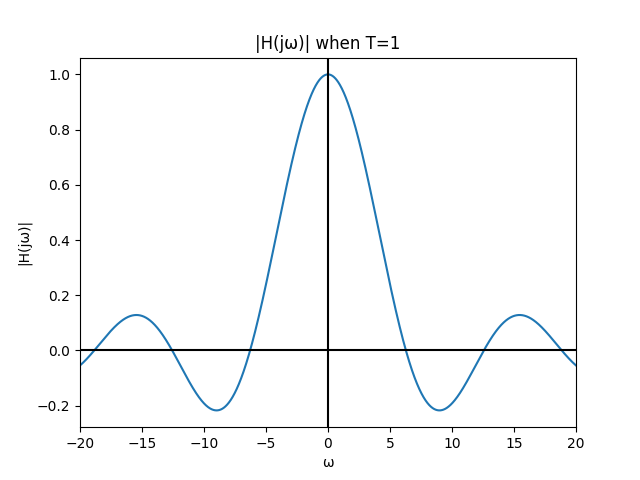
\includegraphics[width=12cm]{img/hw6/mag_plot}

                        $\lim_{\omega \to \infty} |H(j\omega)| = \boxed{0}$.
                  \item The FT of a periodic signal consists of a bunch of impulses
                        where its Fourier coefficients should be.
                        When multiplied with this filter, the inverse FT of the result
                        would be constant iff the result is nonzero at $0$ and nowhere else.

                        Thus, we need the $\frac{\omega_0 T}{2\pi}$ to be an integer,
                        so $\omega_0=\frac{2n\pi}{T}, n \in \mathbb{Z}$, and by extension
                        the period has to be $\boxed{\frac{T}{n}, n \in \mathbb{Z}}$.
                  \item As long the entire frequency stays within the first "mound"
                        of the sinc function, everything should be retained.
                        This mound goes from $\omega=-\frac{2\pi}{T}$ to $\omega=+\frac{2\pi}{T}$,
                        so the maximum value of $B$ we can get is $\boxed{\frac{1}{T}}$.

                        Within this frequency, the group delay is
                        \begin{align*}
                              t_d(\omega)
                               & = -\frac{d}{d\omega} \angle H(j\omega)                \\
                               & = -\frac{d}{d\omega} \left(-\frac{\omega T}{2}\right) \\
                               & = \boxed{\frac{T}{2}}
                        \end{align*}
            \end{enumerate}
      \item \begin{enumerate}
                  \item \begin{enumerate}
                              \item 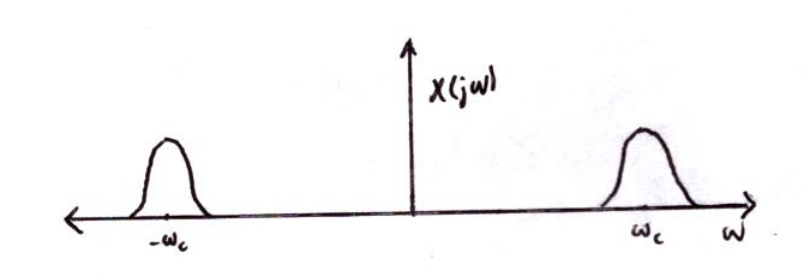
\includegraphics[width=12cm]{img/hw6/x}
                              \item 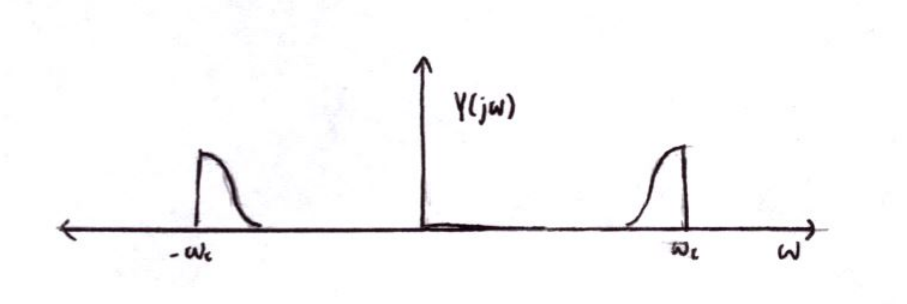
\includegraphics[width=12cm]{img/hw6/y}
                              \item 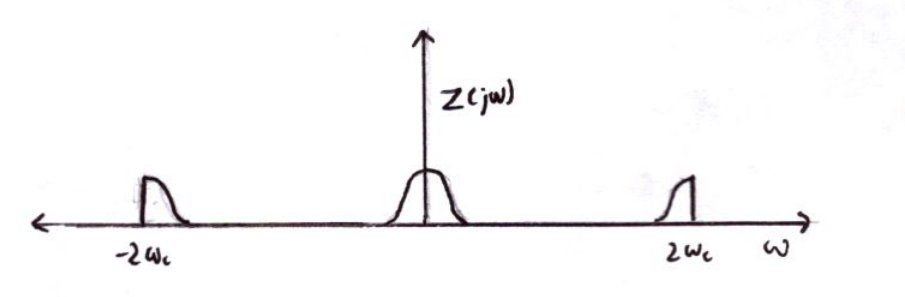
\includegraphics[width=12cm]{img/hw6/z}
                        \end{enumerate}

                        The system recovers $\frac{1}{2}M(j\omega)$.
                        To fully reocver it, just increase the scaling
                        of the LPF by another factor of $2$.
                  \item Samplying in the time domain by multiplication with $\delta_T(t)$
                        is equivalent to convolving in the frequency domain with $\delta_{\omega_0}(\omega)$.

                        $Y(j\omega)$ consists of the right half of the mound at $-\omega_c$
                        and the left half of the mound at $\omega_c$.
                        Convolving with the impulse train makes copies of it
                        shifted $\omega_c$ and $-\omega_c$, which create a mound
                        of half the original height at $\omega=0$.
                        There's other translations too, but they're all filted
                        out by the LPF.

                        This is what the new $Z(j\omega)$ looks like: \\
                        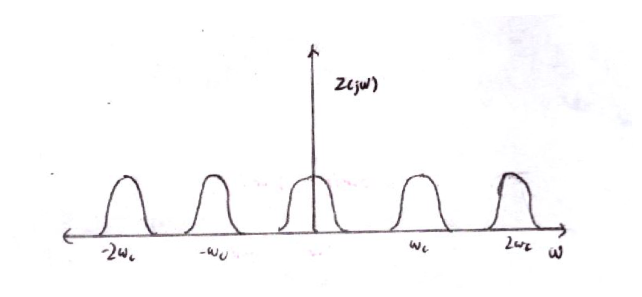
\includegraphics[width=12cm]{img/hw6/sampled_z}
            \end{enumerate}
\end{enumerate}
\end{document}
